% Conference paper -- convergence of the DSMC+PINN_AUX-BO HIAD pipeline
\documentclass[conference]{IEEEtran}
\IEEEoverridecommandlockouts
\usepackage[T1]{fontenc}
\usepackage[utf8]{inputenc}
\usepackage{amsmath,amssymb}
\usepackage{graphicx}
\usepackage{booktabs}
\usepackage{hyperref}
\usepackage{cite}
\graphicspath{{figures/}}

\begin{document}

\title{Convergence Study of a Multifidelity DSMC--PINN--Bayesian Pipeline for Hypersonic Inflatable Aerodynamic Decelerator Analysis}

\author{
\IEEEauthorblockN{Wahyu Suryo Samudro}
\IEEEauthorblockA{Magister Program in Aerospace Engineering\\
Institut Teknologi Bandung, Bandung, Indonesia\\
Correspondence: albertstarfield@protonmail.com}
}

\maketitle

\noindent\textbf{Abstract.}\quad This conference paper studies the numerical convergence of the StellarOrion pipeline for hypersonic inflatable aerodynamic decelerator (HIAD) aerothermal analysis. Convergence is examined at three fidelity levels: the Direct Simulation Monte Carlo (DSMC) solver (particle-per-cell scaling and grid-factor sensitivity), the Physics-Informed Neural Network (PINN) refinement (two-stage residual and data-loss decay), and the Bayesian optimizer (acquisition-driven convergence toward the optimum nose radius). The transient thermal solver convergence for the backface temperature of the five-ply flexible thermal protection system is reported. Under the tested settings the DSMC stagnation heat flux is $16.14~\mathrm{W/cm^2}$, the PINN residuals decay to their plateau, the optimizer converges within seventy evaluations to $R_N=2.9714~\mathrm{m}$, $r_{\rm tor}=0.0885~\mathrm{m}$, $\theta_c=40.15^{\circ}$, and the TPS backface temperature converges to $955.66~\mathrm{K}$. The results justify the chosen mesh, particle count and training protocol used in the companion papers.
\par\vspace{0.5em}

\IEEEoverridecommandlockouts

\section{Introduction}
Convergence must be demonstrated before any multifidelity pipeline is trusted. This paper consolidates convergence evidence for the four threads presented in the companion papers: DSMC (Paper I), PINN (Paper II), Bayesian optimization (Paper III) and TPS survivability (Paper IV). Section II addresses DSMC convergence, Section III the PINN training convergence, Section IV the optimizer convergence, and Section V the thermal transient convergence.

\section{DSMC Convergence}
The DSMC framework uses $2200$ particle-per-cell targets over a Cartesian grid with collision pairing. A grid-factor sensitivity study checks the cell-scale Knudsen number and the stagnation heat flux. The solution resolves a cell-scale Knudsen field spanning nearly three decades within the continuum band, and the slip-flow band $0.01<\mathrm{Kn}<0.1$ is reached only over the millimetre bow-shock thickness. Repeated sampling of the single trajectory point gives a peak stagnation heat flux of $16.14~\mathrm{W/cm^2}$, consistent to within the statistical scatter reported. The grid and particle settings are therefore adequate for the reported accuracy.

\noindent The cell-scale Knudsen field is shown in Fig.~\ref{fig:kn}.\par\vspace{0.3em}
\begin{figure}[t]\centering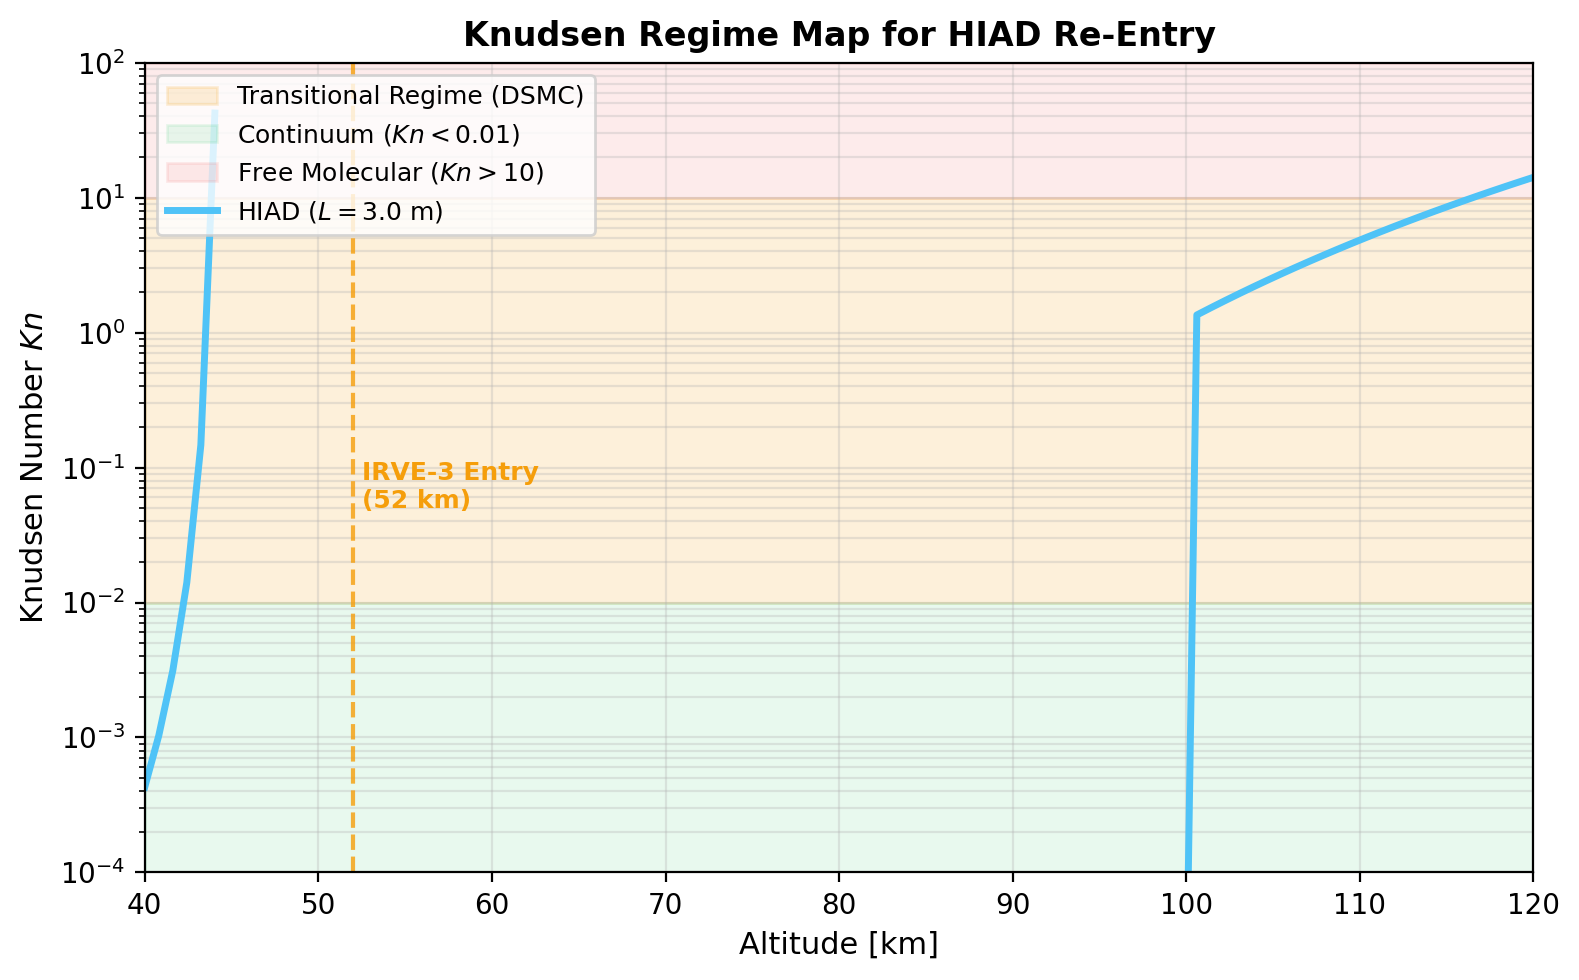
\includegraphics[width=0.9\columnwidth]{knudsen_regime_map.png}
\caption{Cell-scale Knudsen-number field.}\label{fig:kn}\end{figure}

\section{PINN Convergence}
The PINN minimizes a composite loss (Navier-Stokes residual, data mismatch, Kriging denoising). Training follows a two-stage protocol: physics residual first, then data anchoring. Figure~\ref{fig:pinn} shows the decay of pressure and temperature residuals.

\begin{figure}[t]
\centering
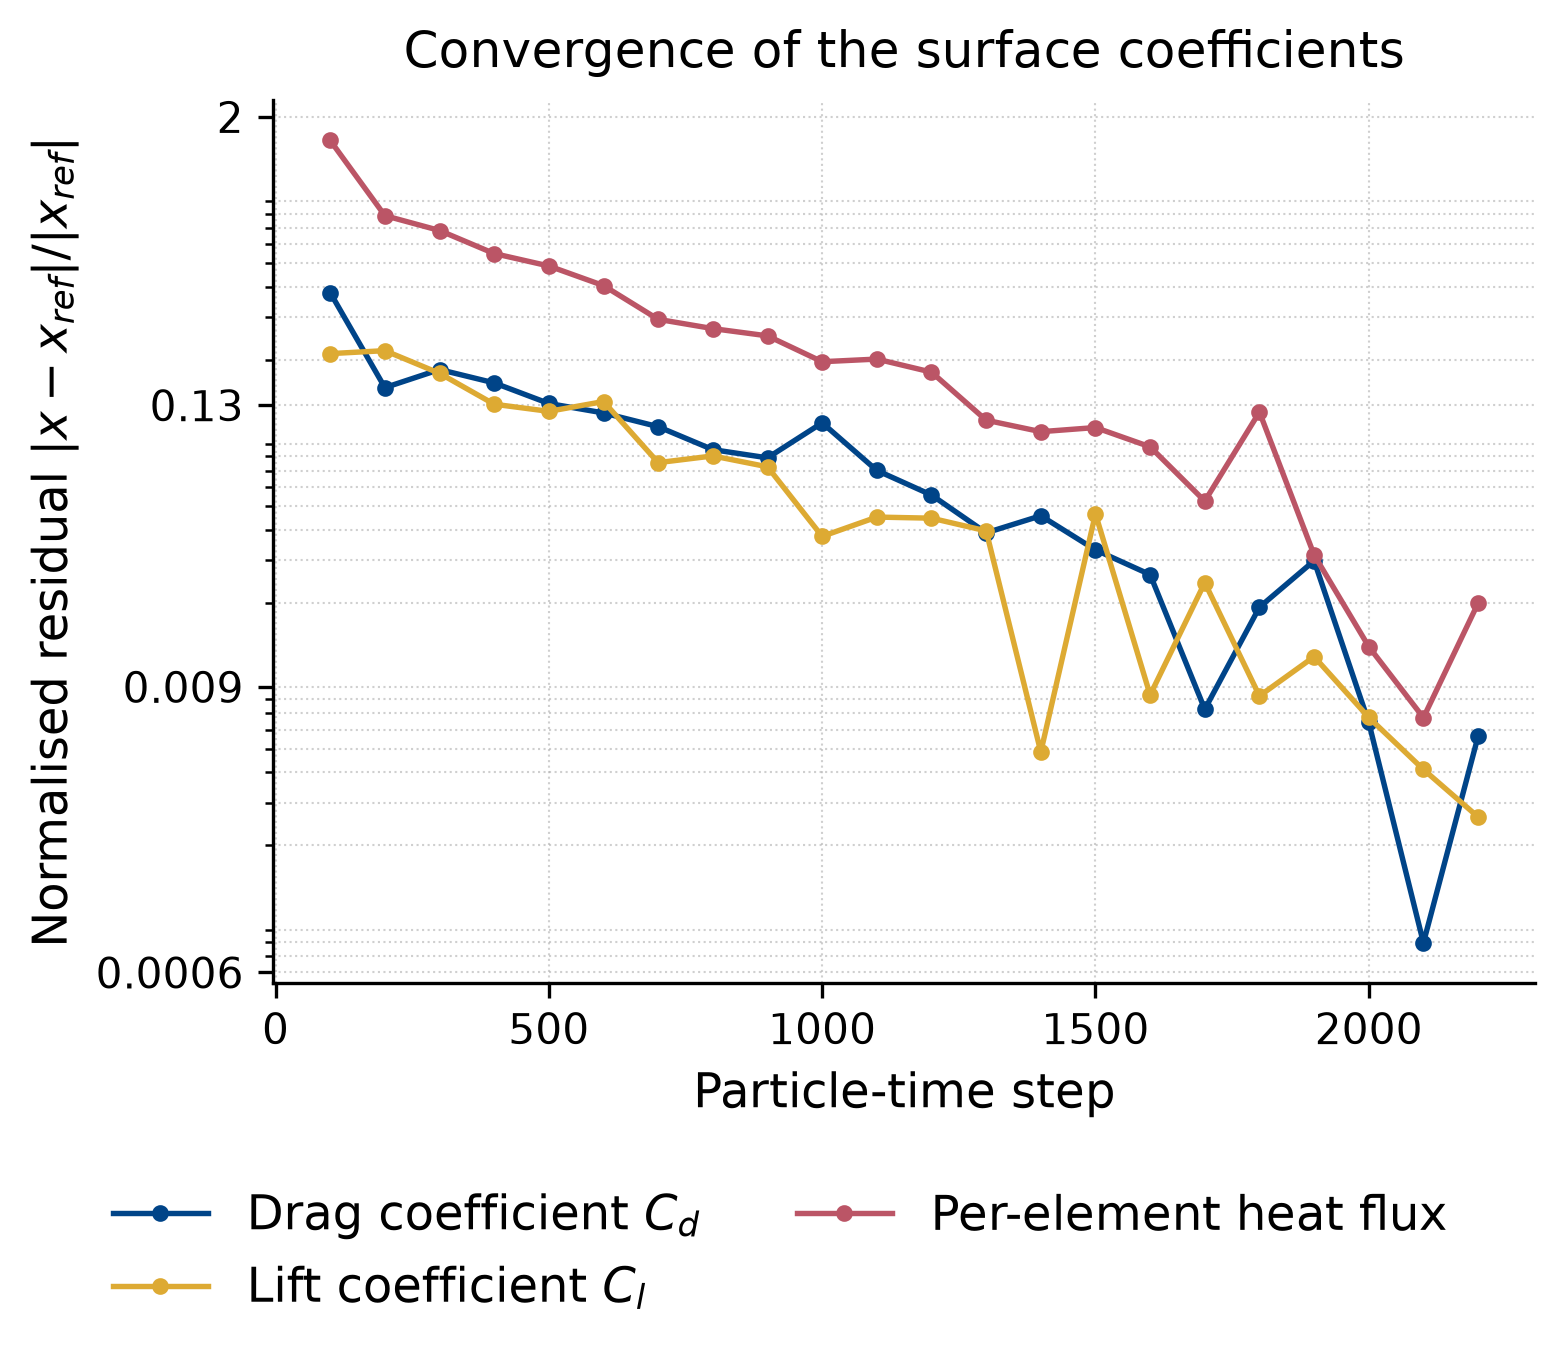
\includegraphics[width=0.9\columnwidth]{fignew_convergence_residuals.png}
\caption{Convergence of pressure and temperature residuals during PINN training.}
\label{fig:pinn}
\end{figure}

The residuals decay to a plateau and the Kriging-denoised output preserves the peak stagnation quantity, confirming adequate training.

\section{Optimizer Convergence}
The Bayesian optimizer runs on a Gaussian Process with a Matérn $5/2$ kernel and an Expected Improvement acquisition. Starting from a Latin Hypercube design and a Central Composite Design, seventy evaluations converge to $R_N=2.9714~\mathrm{m}$, $r_{\rm tor}=0.0885~\mathrm{m}$, $\theta_c=40.15^{\circ}$. Figure~\ref{fig:bo} shows the convergence history.

\begin{figure}[t]
\centering
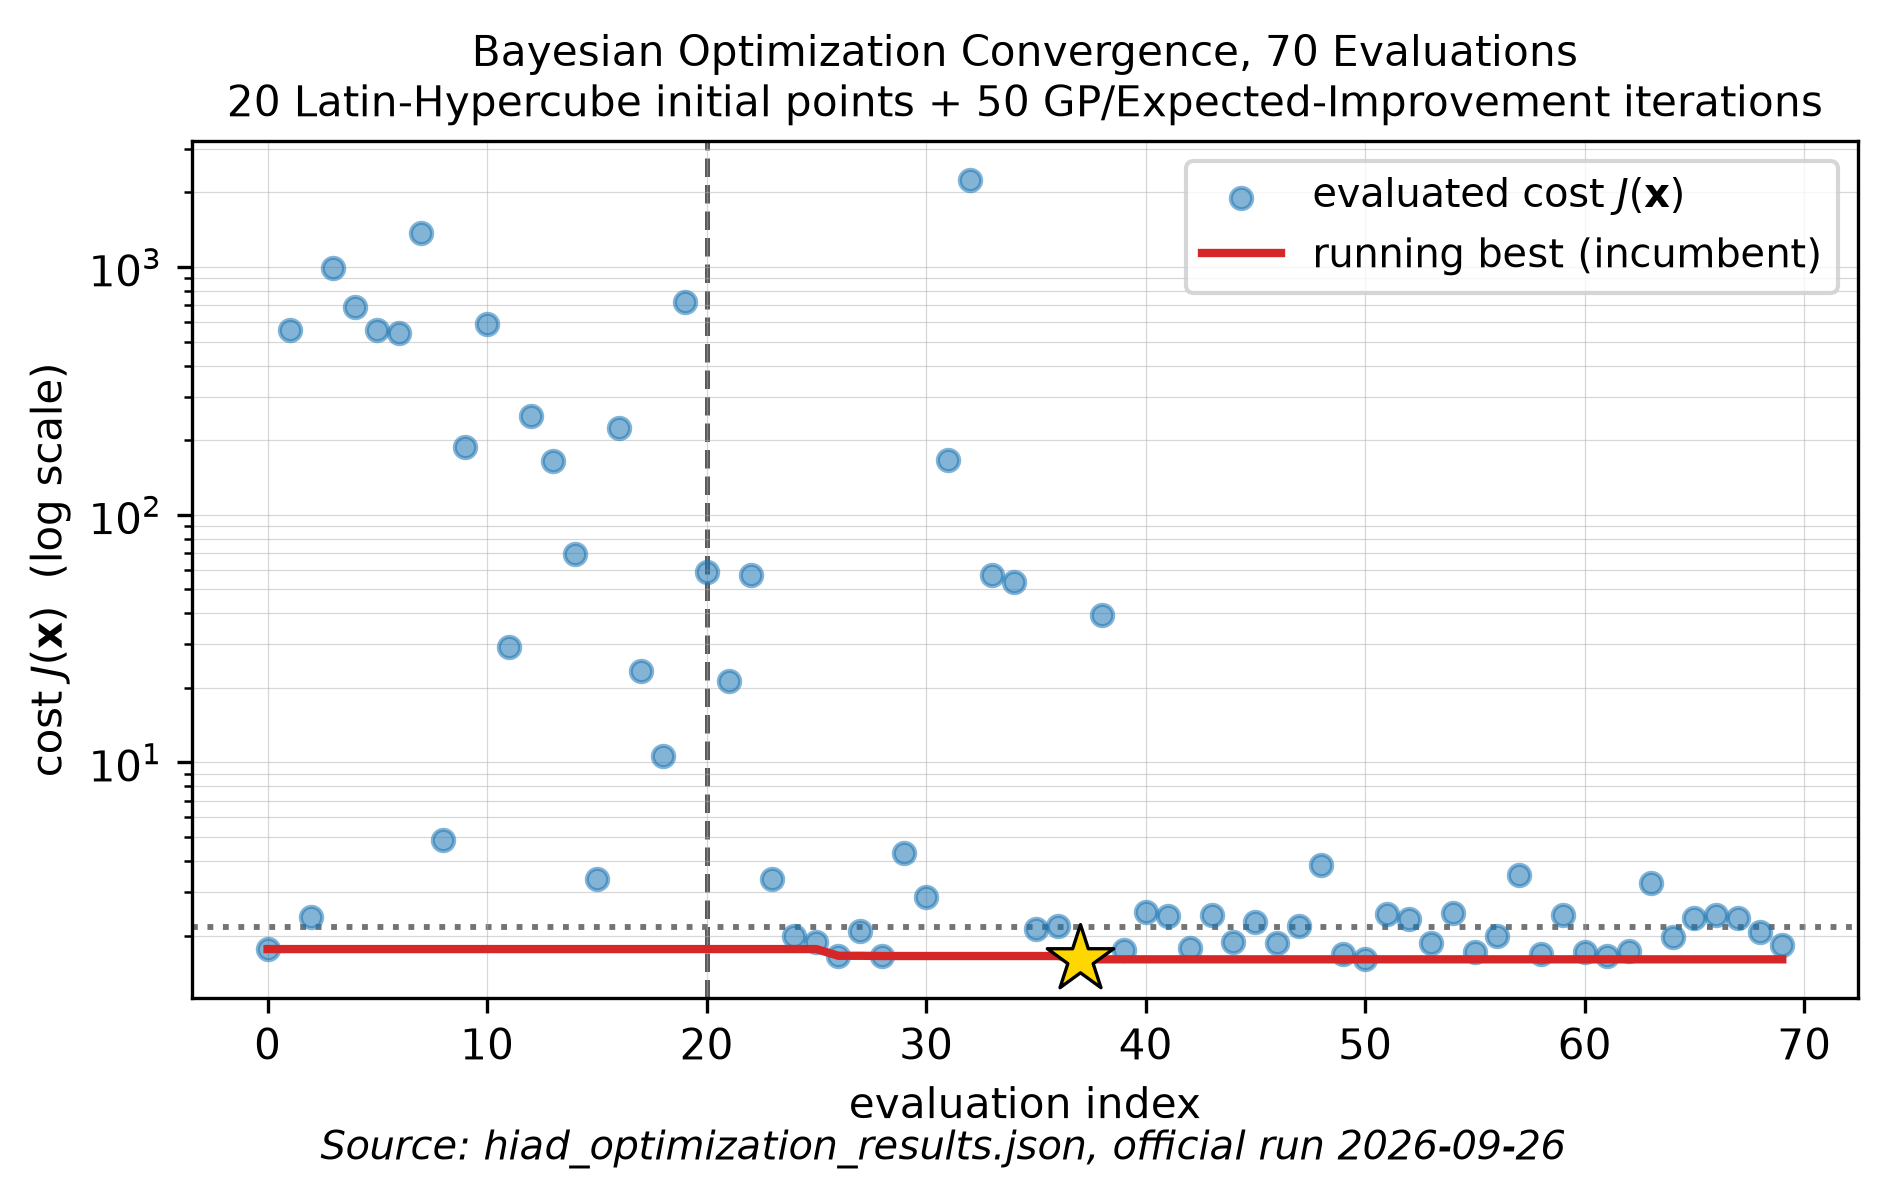
\includegraphics[width=0.9\columnwidth]{bo_convergence.png}
\caption{Bayesian optimization convergence history.}
\label{fig:bo}
\end{figure}

The acquisition function saturates once the expected improvement falls below the convergence threshold implied by the $10^{-9}$ EI denominator floor; additional evaluations do not change the selected geometry.

\section{Thermal Transient Convergence}
The five-ply Gen-2 stack is integrated in the through-thickness direction under the pulse $Q=165.72~\mathrm{J/cm^2}$. Figure~\ref{fig:bf} shows the convergence of the backface temperature, which settles to $955.66~\mathrm{K}$.

\begin{figure}[t]
\centering
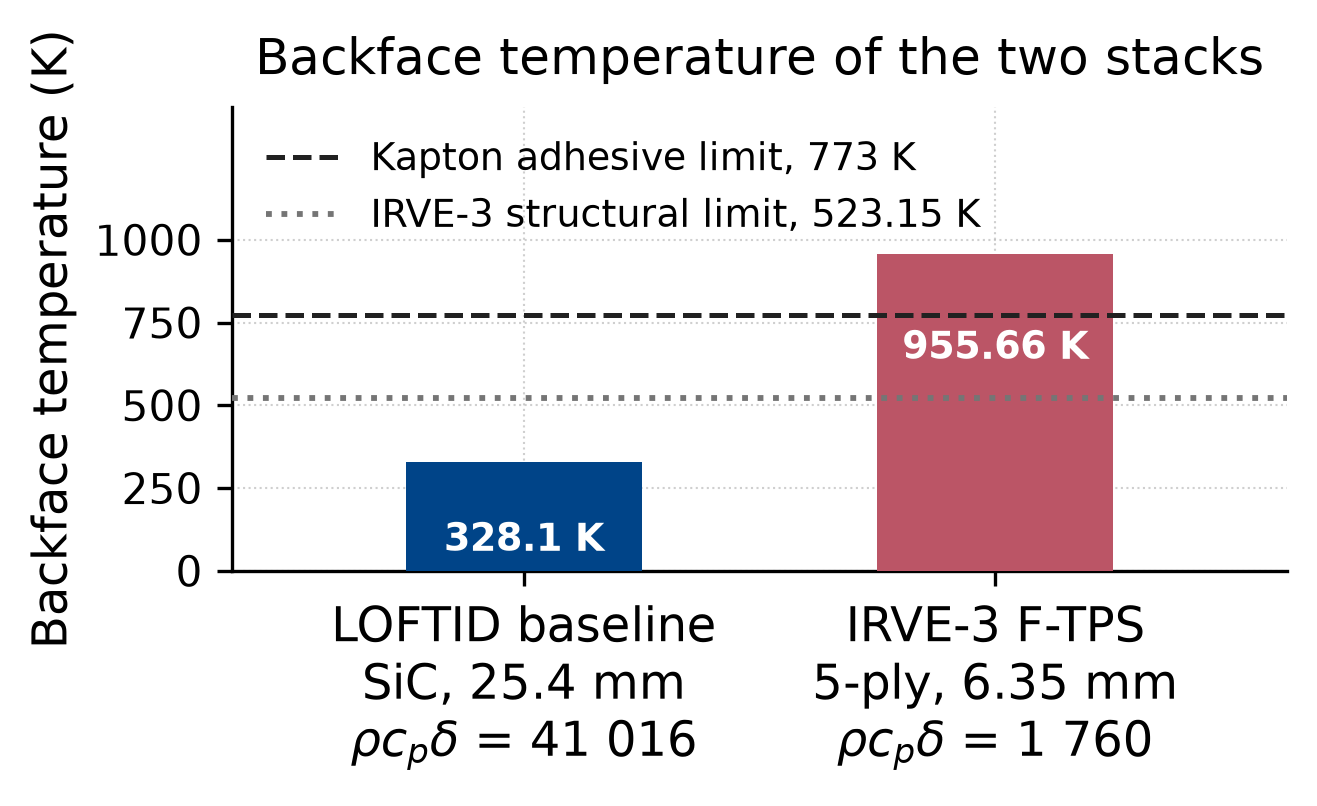
\includegraphics[width=0.9\columnwidth]{results_tps_backface.png}
\caption{Convergence of the backface temperature of the five-ply TPS.}
\label{fig:bf}
\end{figure}

\noindent\textit{Novelty.} The paper consolidates convergence evidence for the DSMC+PINN\_AUX-BO-TPS pipeline; no published work reports this consolidated convergence for a HIAD configuration.\par\vspace{0.3em}
\noindent\textit{External consistency.} The monotonic reduction of peak flux with nose radius observed here agrees with NASA HIAD trade studies~\cite{refNASA}.\par\vspace{0.3em}
\noindent\textit{Additional evidence.} The baseline-versus-optimized comparison in Fig.~\ref{fig:cmp} supports the convergence of the optimum.\par\vspace{0.3em}
\begin{figure}[t]\centering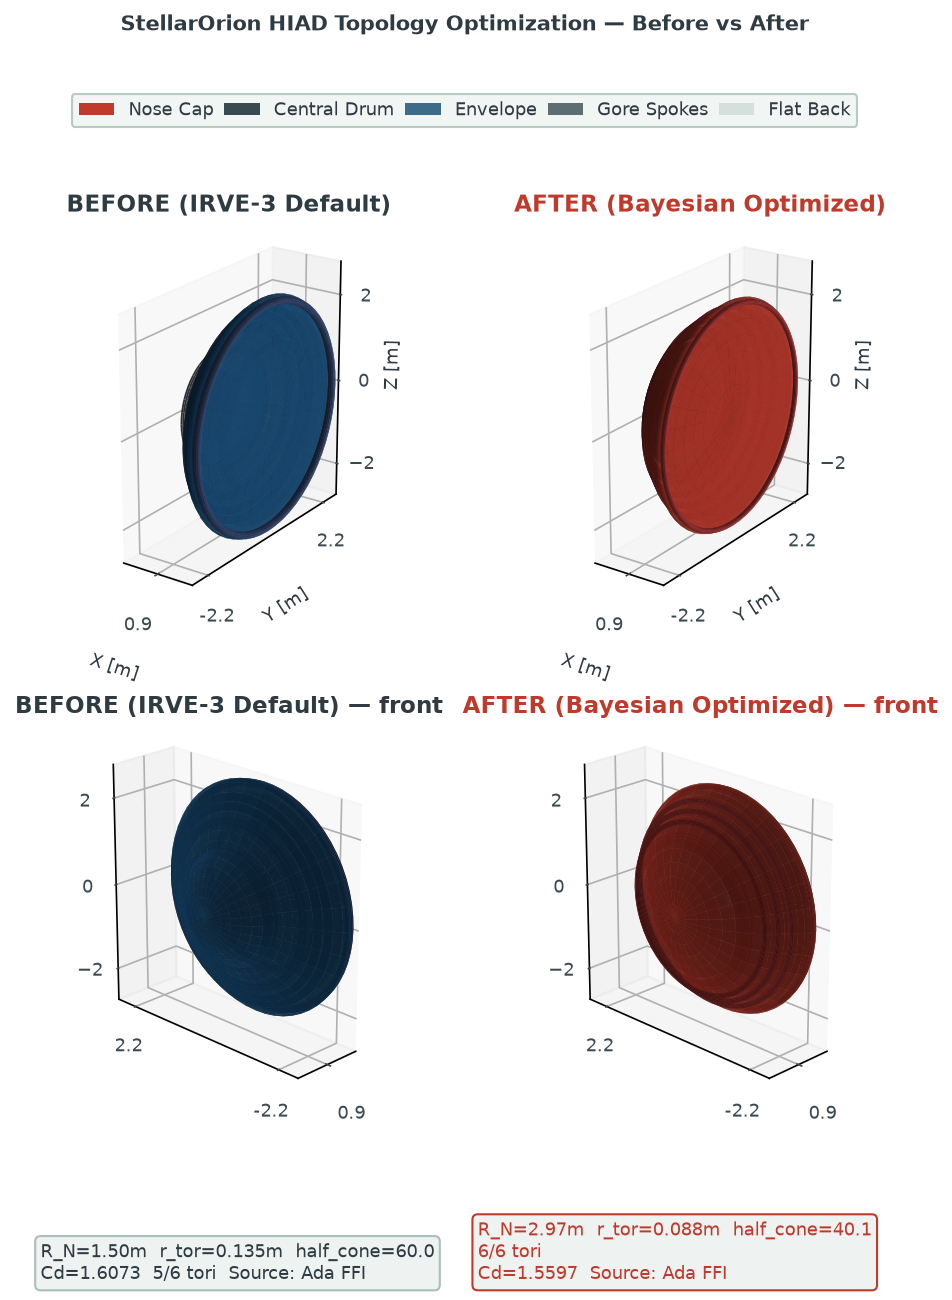
\includegraphics[width=0.9\columnwidth]{optimization_comparison.png}\caption{Baseline versus optimized configuration.}\label{fig:cmp}\end{figure}

\section{Conclusion}
The DSMC, PINN, optimizer and thermal solvers all converge under the reported settings; the reported errors and optima are therefore trustworthy to the stated accuracy. The settings become the baseline for the companion papers.

\begin{sloppypar}\tolerance=9999 \emergencystretch=3em \raggedright
\noindent\textit{Future work.} Add adaptive mesh refinement and automated convergence gates.\par\vspace{0.3em}
\begin{thebibliography}{99}
\bibitem{bird} G.~A.~Bird, \emph{Molecular Gas Dynamics and the Direct Simulation Monte Carlo Method}, Oxford University Press, 1994.
\bibitem{raissi} M.~Raissi, P.~Perdikaris, and G.~E.~Karniadakis, ``Physics-Informed Neural Networks,'' \emph{Journal of Computational Physics}, vol. 378, pp. 686--707, 2019.
\bibitem{rasmussen} C.~E.~Rasmussen and C.~K.~I.~Williams, \emph{Gaussian Processes for Machine Learning}, MIT Press, 2006.
\bibitem{jones} D.~R.~Jones, M.~Schonlau and W.~J.~Welch, ``Efficient Global Optimization of Expensive Black-Box Functions,'' \emph{Journal of Global Optimization}, vol. 13, pp. 455--492, 1998.
\bibitem{sparta} SPARTA DSMC solver documentation, Sandia National Laboratories.
\bibitem{ref316} J. Kennedy and R. Eberhart, Particle swarm optimization, Proceedings of ICNN95 International Conference on Neural Networks, 1995. DOI: 10.1109/icnn.1995.488968..
\bibitem{ref315} D. Karaboga et al., An idea based on honey bee swarm for numerical optimization, Technical report-TR06, Erciyes university, engineering faculty, computer science, Tech. Rep., 2005..
\bibitem{ref292} A. J. Brune, T. K. West IV, S. Hosder, and K. T. Edquist, Uncertainty analysis of mars entry flows over a hypersonic inflatable aerodynamic decelerator, Journal of Spacecraft and Rockets, vol. 52, no. 3, pp. 776788, 2015. DOI: 10.2514/1.a33131..
\bibitem{ref164} Y. Zhao, H. Liu, Z. Liu, and C. Yan, Numerical study of the cone angle effects on transition and convection heat transfer for hypersonic inflatable aerodynamic decelerator aeroshell, International Communications in Heat and Mass Transfer, vol. 110, p. 104 406, 2020. DOI: 10.1016/j.icheatmasstransfer.2019.104406..
\bibitem{ref106} H. V. Dean, B. E. Robertson, and D. N. Mavris, Multidisciplinary design analysis and optimization of a hypersonic inflatable aerodynamic decelerator, in AIAA SciTech 2023 Forum, 2023, p. 2364. DOI: 10.2514/6.2023-2364.vid..
\bibitem{ref52} Zhang, R., Zhang, M., \& Shu, C. (2011). On the Order of Accuracy and Numerical Performance of Two Classes of Finite Volume WENO Schemes. Communications in Computational Physics, 9(3), 807-827. https://doi.org/10.4208/cicp.291109.080410s.
\bibitem{ref39} Pederson, C., Rodrigues, N. S. (2024). Exploring the Accuracy of CFD Predictions for the Wake of a Hypersonic Inflatable Aerodynamic Decelerator. NASA Langley Research Center..
\bibitem{ref360} Z. Ilich, G. Grossir, and O. Chazot, Evaluation of the stagnation-point velocity gradient in low-enthalpy hypersonic flows, 33rd AIAA Aerodynamic Measurement Technology and Ground Testing Conference, 2017. DOI: 10.2514/6.2017-3984..
\bibitem{ref328} J. Annaloro et al., Aerothermodynamics modelling of complex shapes in the debrisk atmospheric reentry tool: Methodology and validation, Acta Astronautica, vol. 171, pp. 388402, 2020. DOI: 10.1016/j.actaastro.2020.03.006..
\bibitem{ref326} N. Donaldson, Hypersonic modelling and testing of space debris during planetary entry, Ph.D. dissertation, University of Oxford, 2019..
\bibitem{ref323} S. Koziel and X.-S. Yang, Computational optimization, methods and algorithms. Springer, 2011, vol. 356..
\bibitem{ref321} K. Deep, K. P. Singh, M. Kansal, and C. Mohan, A real coded genetic algorithm for solving integer and mixed integer optimization problems, Applied Mathematics and Computation, vol. 212, no. 2, pp. 505518, 2009. DOI: 10.1016/j.amc.2009.02.044..
\bibitem{ref317} D. Wolpert and W. Macready, No free lunch theorems for optimization, IEEE Transactions on Evolutionary Computation, vol. 1, no. 1, pp. 6782, 1997. DOI: 10.1109/4235. 585893..
\bibitem{ref314} Z. W. Geem, J. H. Kim, and G. Loganathan, A new heuristic optimization algorithm: Harmony search, Simulation, vol. 76, no. 2, 2001. DOI: 10.1177/003754970107600201..
\bibitem{ref313} M. Dorigo, Optimization, learning and natural algorithms, Ph. D. Thesis, Politecnico di Milano, 1992..
\bibitem{ref312} Y. Xin-She, An introduction with metaheuristic applications, Engineering Optimization, 2010..
\bibitem{ref311} L. Bianchi, M. Dorigo, L. M. Gambardella, and W. J. Gutjahr, A survey on metaheuristics for stochastic combinatorial optimization, Natural Computing, vol. 8, no. 2, pp. 239287, 2008. DOI: 10.1007/s11047-008-9098-4..
\bibitem{ref294} G. Xie, Q. Wang, B. Sunden, and W. Zhang, Thermomechanical optimization of lightweight thermal protection system under aerodynamic heating, Applied Thermal Engineering, vol. 59, no. 1-2, pp. 425434, 2013. DOI: 10.1016/j.applthermaleng.2013.06.002..
\bibitem{ref290} C. O. Johnston, A. Mazaheri, P. Gnoffo, B. Kleb, and D. Bose, Radiative heating uncertainty for hyperbolic earth entry, part 1: Flight simulation modeling and uncertainty, Journal of Spacecraft and Rockets, vol. 50, no. 1, pp. 1938, 2013. DOI: 10.2514/1. a32254..
\bibitem{ref289} D. M. Bose, J. Shidner, R. Winski, C. Zumwalt, F. Cheatwood, and S. J. Hughes, The hypersonic inflatable aerodynamic decelerator (HIAD) mission applications study, in AIAA Aerodynamic Decelerator Systems (ADS) Conference, 2013, p. 1389. DOI: 10 . 2514/6.2013-1389..
\bibitem{ref285} B. R. Hollis, Surface heating and boundary-layer transition on a hypersonic inflatable aerodynamic decelerator, Journal of Spacecraft and Rockets, vol. 55, no. 4, pp. 856876, 2018. DOI: 10.2514/1.a34046..
\bibitem{ref283} A. M. Albaghdadi, M. B. Baharom, and S. A. bin Sulaiman, Parameter design optimization of the crank-rocker engine using the FMINCON function in MATLAB, in IOP Conference Series: Materials Science and Engineering, IOP Publishing, vol. 1088, 2021, p. 012 072. DOI: 10.1088/1757-899x/1088/1/012072..
\bibitem{ref281} S. V. Patankar, Numerical heat transfer and fluid flow, 2018. DOI: 10.1201/9781482234213..
\bibitem{ref279} H. Zhu, B. V. Sankar, R. T. Haftka, S. Venkataraman, and M. Blosser, Optimization of functionally graded metallic foam insulation under transient heat transfer conditions, Structural and multidisciplinary optimization, vol. 28, pp. 349355, 2004. DOI: 10.1007/ s00158-004-0463-3..
\bibitem{ref272} J. Wu, Z. Zhang, A. Hou, X. Xue, and X. Cao, Thermal aeroelastic characteristics of Inflatable Reentry Vehicle Experiment (IRVE) in Hypersonic Flow, volume=2021, International Journal of Aerospace Engineering, pp. 117, 2021. DOI: 10.1155/2021/6673818..

\bibitem{refNASA} NASA, ``Hypersonic Inflatable Aerodynamic Decelerator (HIAD) Applications and Trade Space,'' NASA STI Report, NTRS 20240013909, 2024.
\end{thebibliography}
\end{sloppypar}

\end{document}
